% Options for packages loaded elsewhere
\PassOptionsToPackage{unicode}{hyperref}
\PassOptionsToPackage{hyphens}{url}
%
\documentclass[
]{article}
\title{Practical Work}
\usepackage{etoolbox}
\makeatletter
\providecommand{\subtitle}[1]{% add subtitle to \maketitle
  \apptocmd{\@title}{\par {\large #1 \par}}{}{}
}
\makeatother
\subtitle{Lifetime Data Analysis}
\author{Rodrigo Arriaza, Alexander J Ohrt}
\date{06 December, 2021}

\usepackage{amsmath,amssymb}
\usepackage{lmodern}
\usepackage{iftex}
\ifPDFTeX
  \usepackage[T1]{fontenc}
  \usepackage[utf8]{inputenc}
  \usepackage{textcomp} % provide euro and other symbols
\else % if luatex or xetex
  \usepackage{unicode-math}
  \defaultfontfeatures{Scale=MatchLowercase}
  \defaultfontfeatures[\rmfamily]{Ligatures=TeX,Scale=1}
\fi
% Use upquote if available, for straight quotes in verbatim environments
\IfFileExists{upquote.sty}{\usepackage{upquote}}{}
\IfFileExists{microtype.sty}{% use microtype if available
  \usepackage[]{microtype}
  \UseMicrotypeSet[protrusion]{basicmath} % disable protrusion for tt fonts
}{}
\makeatletter
\@ifundefined{KOMAClassName}{% if non-KOMA class
  \IfFileExists{parskip.sty}{%
    \usepackage{parskip}
  }{% else
    \setlength{\parindent}{0pt}
    \setlength{\parskip}{6pt plus 2pt minus 1pt}}
}{% if KOMA class
  \KOMAoptions{parskip=half}}
\makeatother
\usepackage{xcolor}
\IfFileExists{xurl.sty}{\usepackage{xurl}}{} % add URL line breaks if available
\IfFileExists{bookmark.sty}{\usepackage{bookmark}}{\usepackage{hyperref}}
\hypersetup{
  pdftitle={Practical Work},
  pdfauthor={Rodrigo Arriaza, Alexander J Ohrt},
  hidelinks,
  pdfcreator={LaTeX via pandoc}}
\urlstyle{same} % disable monospaced font for URLs
\usepackage[margin=1in]{geometry}
\usepackage{color}
\usepackage{fancyvrb}
\newcommand{\VerbBar}{|}
\newcommand{\VERB}{\Verb[commandchars=\\\{\}]}
\DefineVerbatimEnvironment{Highlighting}{Verbatim}{commandchars=\\\{\}}
% Add ',fontsize=\small' for more characters per line
\usepackage{framed}
\definecolor{shadecolor}{RGB}{248,248,248}
\newenvironment{Shaded}{\begin{snugshade}}{\end{snugshade}}
\newcommand{\AlertTok}[1]{\textcolor[rgb]{0.94,0.16,0.16}{#1}}
\newcommand{\AnnotationTok}[1]{\textcolor[rgb]{0.56,0.35,0.01}{\textbf{\textit{#1}}}}
\newcommand{\AttributeTok}[1]{\textcolor[rgb]{0.77,0.63,0.00}{#1}}
\newcommand{\BaseNTok}[1]{\textcolor[rgb]{0.00,0.00,0.81}{#1}}
\newcommand{\BuiltInTok}[1]{#1}
\newcommand{\CharTok}[1]{\textcolor[rgb]{0.31,0.60,0.02}{#1}}
\newcommand{\CommentTok}[1]{\textcolor[rgb]{0.56,0.35,0.01}{\textit{#1}}}
\newcommand{\CommentVarTok}[1]{\textcolor[rgb]{0.56,0.35,0.01}{\textbf{\textit{#1}}}}
\newcommand{\ConstantTok}[1]{\textcolor[rgb]{0.00,0.00,0.00}{#1}}
\newcommand{\ControlFlowTok}[1]{\textcolor[rgb]{0.13,0.29,0.53}{\textbf{#1}}}
\newcommand{\DataTypeTok}[1]{\textcolor[rgb]{0.13,0.29,0.53}{#1}}
\newcommand{\DecValTok}[1]{\textcolor[rgb]{0.00,0.00,0.81}{#1}}
\newcommand{\DocumentationTok}[1]{\textcolor[rgb]{0.56,0.35,0.01}{\textbf{\textit{#1}}}}
\newcommand{\ErrorTok}[1]{\textcolor[rgb]{0.64,0.00,0.00}{\textbf{#1}}}
\newcommand{\ExtensionTok}[1]{#1}
\newcommand{\FloatTok}[1]{\textcolor[rgb]{0.00,0.00,0.81}{#1}}
\newcommand{\FunctionTok}[1]{\textcolor[rgb]{0.00,0.00,0.00}{#1}}
\newcommand{\ImportTok}[1]{#1}
\newcommand{\InformationTok}[1]{\textcolor[rgb]{0.56,0.35,0.01}{\textbf{\textit{#1}}}}
\newcommand{\KeywordTok}[1]{\textcolor[rgb]{0.13,0.29,0.53}{\textbf{#1}}}
\newcommand{\NormalTok}[1]{#1}
\newcommand{\OperatorTok}[1]{\textcolor[rgb]{0.81,0.36,0.00}{\textbf{#1}}}
\newcommand{\OtherTok}[1]{\textcolor[rgb]{0.56,0.35,0.01}{#1}}
\newcommand{\PreprocessorTok}[1]{\textcolor[rgb]{0.56,0.35,0.01}{\textit{#1}}}
\newcommand{\RegionMarkerTok}[1]{#1}
\newcommand{\SpecialCharTok}[1]{\textcolor[rgb]{0.00,0.00,0.00}{#1}}
\newcommand{\SpecialStringTok}[1]{\textcolor[rgb]{0.31,0.60,0.02}{#1}}
\newcommand{\StringTok}[1]{\textcolor[rgb]{0.31,0.60,0.02}{#1}}
\newcommand{\VariableTok}[1]{\textcolor[rgb]{0.00,0.00,0.00}{#1}}
\newcommand{\VerbatimStringTok}[1]{\textcolor[rgb]{0.31,0.60,0.02}{#1}}
\newcommand{\WarningTok}[1]{\textcolor[rgb]{0.56,0.35,0.01}{\textbf{\textit{#1}}}}
\usepackage{longtable,booktabs,array}
\usepackage{calc} % for calculating minipage widths
% Correct order of tables after \paragraph or \subparagraph
\usepackage{etoolbox}
\makeatletter
\patchcmd\longtable{\par}{\if@noskipsec\mbox{}\fi\par}{}{}
\makeatother
% Allow footnotes in longtable head/foot
\IfFileExists{footnotehyper.sty}{\usepackage{footnotehyper}}{\usepackage{footnote}}
\makesavenoteenv{longtable}
\usepackage{graphicx}
\makeatletter
\def\maxwidth{\ifdim\Gin@nat@width>\linewidth\linewidth\else\Gin@nat@width\fi}
\def\maxheight{\ifdim\Gin@nat@height>\textheight\textheight\else\Gin@nat@height\fi}
\makeatother
% Scale images if necessary, so that they will not overflow the page
% margins by default, and it is still possible to overwrite the defaults
% using explicit options in \includegraphics[width, height, ...]{}
\setkeys{Gin}{width=\maxwidth,height=\maxheight,keepaspectratio}
% Set default figure placement to htbp
\makeatletter
\def\fps@figure{htbp}
\makeatother
\setlength{\emergencystretch}{3em} % prevent overfull lines
\providecommand{\tightlist}{%
  \setlength{\itemsep}{0pt}\setlength{\parskip}{0pt}}
\setcounter{secnumdepth}{-\maxdimen} % remove section numbering
\usepackage{booktabs}
\usepackage{longtable}
\usepackage{array}
\usepackage{multirow}
\usepackage{wrapfig}
\usepackage{float}
\usepackage{colortbl}
\usepackage{pdflscape}
\usepackage{tabu}
\usepackage{threeparttable}
\usepackage{threeparttablex}
\usepackage[normalem]{ulem}
\usepackage{makecell}
\usepackage{xcolor}
\ifLuaTeX
  \usepackage{selnolig}  % disable illegal ligatures
\fi

\begin{document}
\maketitle

\hypertarget{introduction}{%
\section{Introduction}\label{introduction}}

We are given a data set on sexually transmitted diseases (STDs). This is data from a study about gonorrhea and chlamydia in 877 women. The objective with this practical work is to study possible risk factors for a reinfection with gonorrhea or chlamydia in women who have suffered one of both infections previously. The variables of interest are sociodemographic variables or those related to sexual practice. We have a lot of variables at our disposal, as can be seen from the data set below. We have chosen to use the following:

\begin{itemize}
\tightlist
\item
  NumPartners: The number of partners during the last 30 days.
\item
  CondomUse: Use of condoms (1: always, 2: once in a while, 3: never)
\item
  YearsSchool: Years of schooling.
\item
  InitInfect: Initial infection (1: Gonorrhea, 2: Chlamydia, 3: both)
\item
  NumPartners: Number of sexual partners during the last 30 days.
\item
  InvVagAtExam: Involvement vagina at exam (1: yes; 0: no).
\item
  DischargeExam: Discharge at exam (1: yes; 0: no)
\end{itemize}

The first two were chosen based on results from a \href{https://www.ncbi.nlm.nih.gov/pmc/articles/PMC1744639/}{study} on gonorrhea reinfection in heterosexual STD clinic attendees. The study concluded that increased reinfection risk (of gonorrhea) was associated with younger age and a greater number of recent sex partners, among other risk factors. Moreover, the authors concluded that any type of condom use was a risk factor for reinfection with gonorrhea in women. However by using statistical analysis we found that the Age of the woman and the ethnicity (a variable that was included in the forementioned study) are not statistically significant.

Another \href{https://policylab.chop.edu/sites/default/files/pdf/publications/Preventing_Chlamydia_Gonorrhea_Reinfection_through_Increased_Use_of_EPT.pdf}{publication} reports that, on average, 14\% of women with clamydia and 12\% of women with gonorrhea get reinfected, with younger women at higher risk. Moreover, they state that many adolescents treated for infection of one of the two STDs are reinfected within three to six months, usually because of resumed sexual contact with an untreated partner. Thus, the marital status might be interesting to analyse. However, this is not added after all, because, as seen in the exploratory data analysis below, the ages are low, which should mean that the amount in each level of \texttt{MaritalStatus} is very skewed towards single. This can be seen in the table below as well.

\href{https://www.ncbi.nlm.nih.gov/pmc/articles/PMC2094865/}{This meta-analysis} reports that the relationship between race, socioeconomic status (SES) and chlamydial infection is not clear. It concludes that SES was not associated with chlamydia infection, where they tested for several variables, where level of parent's education was one of them. Either way, we think it might be interesting to see if the years of schooling of the women have any impact on chlamyida reinfection and as is shown below it showed to be statistically significant during the exploratory analysis.

\begin{Shaded}
\begin{Highlighting}[]
\NormalTok{std\_data }\OtherTok{\textless{}{-}} \FunctionTok{read.table}\NormalTok{(}\StringTok{"STD\_onlydata.txt"}\NormalTok{)}
\FunctionTok{colnames}\NormalTok{(std\_data) }\OtherTok{\textless{}{-}}\NormalTok{ variable.names }\OtherTok{\textless{}{-}} \FunctionTok{c}\NormalTok{(}\StringTok{"ObsNum"}\NormalTok{, }\StringTok{"Ethnicity"}\NormalTok{, }\StringTok{"MaritalStatus"}\NormalTok{, }\StringTok{"Age"}\NormalTok{, }\StringTok{"YearsSchool"}\NormalTok{, }\StringTok{"InitInfect"}\NormalTok{, }\StringTok{"NumPartners"}\NormalTok{, }\StringTok{"OralSex12m"}\NormalTok{, }\StringTok{"OralSex30d"}\NormalTok{, }\StringTok{"RectalSex12m"}\NormalTok{, }\StringTok{"RectalSex30d"}\NormalTok{, }\StringTok{"AbPain"}\NormalTok{, }\StringTok{"SignDischarge"}\NormalTok{,}\StringTok{"SignDysuria"}\NormalTok{,}\StringTok{"CondomUse"}\NormalTok{,}\StringTok{"SignItch"}\NormalTok{,}\StringTok{"SignLesion"}\NormalTok{,}\StringTok{"SignRash"}\NormalTok{,}\StringTok{"SignLymph"}\NormalTok{,}\StringTok{"InvVagAtExam"}\NormalTok{,}\StringTok{"DischargeExam"}\NormalTok{,}\StringTok{"AbnormNodeExam"}\NormalTok{, }\StringTok{"Reinfection"}\NormalTok{, }\StringTok{"TimeUntilReinf"}\NormalTok{)}

\NormalTok{std\_data[, variable.names[}\SpecialCharTok{{-}}\FunctionTok{c}\NormalTok{(}\DecValTok{1}\NormalTok{, }\DecValTok{4}\NormalTok{, }\DecValTok{5}\NormalTok{, }\DecValTok{7}\NormalTok{,}\DecValTok{23}\NormalTok{,}\DecValTok{24}\NormalTok{)]] }\OtherTok{\textless{}{-}} \FunctionTok{lapply}\NormalTok{(std\_data[, variable.names[}\SpecialCharTok{{-}}\FunctionTok{c}\NormalTok{(}\DecValTok{1}\NormalTok{,}\DecValTok{4}\NormalTok{,}\DecValTok{5}\NormalTok{,}\DecValTok{7}\NormalTok{,}\DecValTok{23}\NormalTok{,}\DecValTok{24}\NormalTok{)]],factor)}
\NormalTok{std\_data}\SpecialCharTok{$}\NormalTok{cens }\OtherTok{\textless{}{-}} \FunctionTok{rep}\NormalTok{(}\DecValTok{1}\NormalTok{, }\AttributeTok{length =} \FunctionTok{dim}\NormalTok{(std\_data)[[}\DecValTok{1}\NormalTok{]]) }\CommentTok{\# All uncensored, thus cens = 1 for all rows. }

\NormalTok{variables.chosen }\OtherTok{\textless{}{-}} \FunctionTok{c}\NormalTok{(}\StringTok{"Age"}\NormalTok{, }\StringTok{"NumPartners"}\NormalTok{, }\StringTok{"CondomUse"}\NormalTok{, }\StringTok{"Ethnicity"}\NormalTok{) }\CommentTok{\# ETC!}
\NormalTok{continuous.variables }\OtherTok{\textless{}{-}} \FunctionTok{unlist}\NormalTok{(}\FunctionTok{lapply}\NormalTok{(std\_data, is.numeric))}
\NormalTok{continuous.variables }\OtherTok{\textless{}{-}}\NormalTok{ continuous.variables[}\SpecialCharTok{{-}}\FunctionTok{length}\NormalTok{(continuous.variables)] }\CommentTok{\# Removing the cens{-}value. }
\end{Highlighting}
\end{Shaded}

Naturally, the categorical variable which states if the woman is reinfected or not (\texttt{Reinfection}) will be used as a dependent variable in the analysis and the time until reinfection since the more time a subject is under study, the greater the risk of the event reocurring.

\hypertarget{descriptive-analysis}{%
\section{Descriptive Analysis}\label{descriptive-analysis}}

\hypertarget{variable-selection}{%
\subsection{Variable selection}\label{variable-selection}}

\begin{Shaded}
\begin{Highlighting}[]
\NormalTok{std\_data}\SpecialCharTok{$}\NormalTok{Ethnicity }\OtherTok{\textless{}{-}} \FunctionTok{factor}\NormalTok{(std\_data}\SpecialCharTok{$}\NormalTok{Ethnicity)}
\NormalTok{nb.model }\OtherTok{\textless{}{-}}\NormalTok{ MASS}\SpecialCharTok{::}\FunctionTok{glm.nb}\NormalTok{(Reinfection }\SpecialCharTok{\textasciitilde{}}\NormalTok{ Ethnicity }\SpecialCharTok{+}\NormalTok{ MaritalStatus }\SpecialCharTok{+}\NormalTok{ Age }\SpecialCharTok{+}\NormalTok{ YearsSchool }\SpecialCharTok{+}\NormalTok{ InitInfect }\SpecialCharTok{+}
\NormalTok{                           NumPartners }\SpecialCharTok{+}\NormalTok{OralSex12m }\SpecialCharTok{+}\NormalTok{ OralSex30d }\SpecialCharTok{+}\NormalTok{ RectalSex12m }\SpecialCharTok{+}\NormalTok{ RectalSex30d }\SpecialCharTok{+}\NormalTok{ AbPain }\SpecialCharTok{+}
\NormalTok{               SignDischarge }\SpecialCharTok{+}\NormalTok{ SignDysuria}\SpecialCharTok{+}\NormalTok{ CondomUse }\SpecialCharTok{+}\NormalTok{ SignItch }\SpecialCharTok{+}\NormalTok{ SignLesion }\SpecialCharTok{+}\NormalTok{ SignRash }\SpecialCharTok{+}
\NormalTok{               SignLymph }\SpecialCharTok{+}\NormalTok{ InvVagAtExam }\SpecialCharTok{+}\NormalTok{ DischargeExam }\SpecialCharTok{+}\NormalTok{ AbnormNodeExam }\SpecialCharTok{+} \FunctionTok{offset}\NormalTok{(}\FunctionTok{log}\NormalTok{(TimeUntilReinf)),}
             \AttributeTok{data=}\NormalTok{std\_data)}
\NormalTok{s }\OtherTok{\textless{}{-}} \FunctionTok{summary}\NormalTok{(nb.model)}
\NormalTok{k }\OtherTok{\textless{}{-}}\NormalTok{ knitr}\SpecialCharTok{::}\FunctionTok{kable}\NormalTok{(s}\SpecialCharTok{$}\NormalTok{coefficients, }\AttributeTok{caption =} \StringTok{\textquotesingle{}Variables statistical significance\textquotesingle{}}\NormalTok{)}
\NormalTok{kableExtra}\SpecialCharTok{::}\FunctionTok{row\_spec}\NormalTok{(k, }\FunctionTok{c}\NormalTok{(}\DecValTok{6}\SpecialCharTok{:}\DecValTok{9}\NormalTok{,}\DecValTok{14}\NormalTok{,}\DecValTok{16}\NormalTok{,}\DecValTok{23}\NormalTok{,}\DecValTok{24}\NormalTok{), }\AttributeTok{color=}\StringTok{\textquotesingle{}white\textquotesingle{}}\NormalTok{, }\AttributeTok{background =} \StringTok{\textquotesingle{}cyan\textquotesingle{}}\NormalTok{)}
\end{Highlighting}
\end{Shaded}

\begin{table}

\caption{\label{tab:variable-select}Variables statistical significance}
\centering
\begin{tabular}[t]{l|r|r|r|r}
\hline
  & Estimate & Std. Error & z value & Pr(>|z|)\\
\hline
(Intercept) & -4.4766626 & 0.6791361 & -6.5917022 & 0.0000000\\
\hline
EthnicityW & -0.0786114 & 0.1576156 & -0.4987540 & 0.6179527\\
\hline
MaritalStatusM & 0.1142920 & 0.4681139 & 0.2441542 & 0.8071114\\
\hline
MaritalStatusS & 0.5011754 & 0.3203698 & 1.5643657 & 0.1177317\\
\hline
Age & 0.0188481 & 0.0156143 & 1.2071011 & 0.2273932\\
\hline
\cellcolor{cyan}{\textcolor{white}{YearsSchool}} & \cellcolor{cyan}{\textcolor{white}{-0.1689015}} & \cellcolor{cyan}{\textcolor{white}{0.0442657}} & \cellcolor{cyan}{\textcolor{white}{-3.8156308}} & \cellcolor{cyan}{\textcolor{white}{0.0001358}}\\
\hline
\cellcolor{cyan}{\textcolor{white}{InitInfect2}} & \cellcolor{cyan}{\textcolor{white}{-0.3302518}} & \cellcolor{cyan}{\textcolor{white}{0.1740868}} & \cellcolor{cyan}{\textcolor{white}{-1.8970524}} & \cellcolor{cyan}{\textcolor{white}{0.0578210}}\\
\hline
\cellcolor{cyan}{\textcolor{white}{InitInfect3}} & \cellcolor{cyan}{\textcolor{white}{-0.3318821}} & \cellcolor{cyan}{\textcolor{white}{0.1755787}} & \cellcolor{cyan}{\textcolor{white}{-1.8902183}} & \cellcolor{cyan}{\textcolor{white}{0.0587288}}\\
\hline
\cellcolor{cyan}{\textcolor{white}{NumPartners}} & \cellcolor{cyan}{\textcolor{white}{0.1164568}} & \cellcolor{cyan}{\textcolor{white}{0.0598373}} & \cellcolor{cyan}{\textcolor{white}{1.9462257}} & \cellcolor{cyan}{\textcolor{white}{0.0516276}}\\
\hline
OralSex12m1 & -0.3703474 & 0.2387666 & -1.5510855 & 0.1208812\\
\hline
OralSex30d1 & -0.3246975 & 0.2643311 & -1.2283739 & 0.2193066\\
\hline
RectalSex12m1 & 0.0669703 & 0.4881503 & 0.1371920 & 0.8908790\\
\hline
RectalSex30d1 & -0.1627456 & 0.6172379 & -0.2636675 & 0.7920361\\
\hline
\cellcolor{cyan}{\textcolor{white}{AbPain1}} & \cellcolor{cyan}{\textcolor{white}{0.2969178}} & \cellcolor{cyan}{\textcolor{white}{0.1771403}} & \cellcolor{cyan}{\textcolor{white}{1.6761734}} & \cellcolor{cyan}{\textcolor{white}{0.0937042}}\\
\hline
SignDischarge1 & 0.1330009 & 0.1306664 & 1.0178660 & 0.3087416\\
\hline
\cellcolor{cyan}{\textcolor{white}{SignDysuria1}} & \cellcolor{cyan}{\textcolor{white}{0.1954606}} & \cellcolor{cyan}{\textcolor{white}{0.1812469}} & \cellcolor{cyan}{\textcolor{white}{1.0784219}} & \cellcolor{cyan}{\textcolor{white}{0.2808455}}\\
\hline
CondomUse2 & -0.1553543 & 0.2725108 & -0.5700849 & 0.5686201\\
\hline
CondomUse3 & -0.4582270 & 0.2819913 & -1.6249684 & 0.1041693\\
\hline
SignItch1 & -0.2209724 & 0.1750560 & -1.2622958 & 0.2068424\\
\hline
SignLesion1 & -0.2541307 & 0.3787052 & -0.6710513 & 0.5021878\\
\hline
SignRash1 & -0.0638066 & 0.4592994 & -0.1389215 & 0.8895122\\
\hline
SignLymph1 & 0.2368538 & 0.5922357 & 0.3999317 & 0.6892069\\
\hline
\cellcolor{cyan}{\textcolor{white}{InvVagAtExam1}} & \cellcolor{cyan}{\textcolor{white}{0.5726933}} & \cellcolor{cyan}{\textcolor{white}{0.2003764}} & \cellcolor{cyan}{\textcolor{white}{2.8580874}} & \cellcolor{cyan}{\textcolor{white}{0.0042620}}\\
\hline
\cellcolor{cyan}{\textcolor{white}{DischargeExam1}} & \cellcolor{cyan}{\textcolor{white}{-0.5805191}} & \cellcolor{cyan}{\textcolor{white}{0.2691414}} & \cellcolor{cyan}{\textcolor{white}{-2.1569301}} & \cellcolor{cyan}{\textcolor{white}{0.0310111}}\\
\hline
AbnormNodeExam1 & 0.0801562 & 0.5157541 & 0.1554155 & 0.8764938\\
\hline
\end{tabular}
\end{table}

Note that age and years of schooling are somewhat correlated. \textbf{Could do some more EDA probably, and should remove some of this also.}

\hypertarget{nonparametric-analysis}{%
\section{Nonparametric Analysis}\label{nonparametric-analysis}}

The survival curve is estimated by means of Kaplan-Meier and plotted below. The curve below shows the general survival in the data set, i.e.~not depending on any specific explanatory variable.

\begin{Shaded}
\begin{Highlighting}[]
\NormalTok{s1 }\OtherTok{\textless{}{-}} \FunctionTok{with}\NormalTok{(std\_data, }\FunctionTok{Surv}\NormalTok{(TimeUntilReinf, cens) }\SpecialCharTok{\textasciitilde{}} \DecValTok{1}\NormalTok{)}
\NormalTok{s1fit }\OtherTok{\textless{}{-}} \FunctionTok{survfit}\NormalTok{(s1)}
\CommentTok{\#plot(s1fit)}

\FunctionTok{par}\NormalTok{(}\AttributeTok{font =} \DecValTok{2}\NormalTok{, }\AttributeTok{font.axis =} \DecValTok{2}\NormalTok{, }\AttributeTok{font.lab =} \DecValTok{2}\NormalTok{, }\AttributeTok{las =} \DecValTok{1}\NormalTok{, }\AttributeTok{mar =} \FunctionTok{c}\NormalTok{(}\DecValTok{5}\NormalTok{, }\DecValTok{5}\NormalTok{, }\DecValTok{4}\NormalTok{, }\DecValTok{2}\NormalTok{))}
\FunctionTok{plot}\NormalTok{(s1fit, }\AttributeTok{col =} \DecValTok{2}\NormalTok{, }\AttributeTok{xlab =} \StringTok{"Time to reinfection [days]"}\NormalTok{,}
     \AttributeTok{ylab =} \FunctionTok{expression}\NormalTok{(}\FunctionTok{bolditalic}\NormalTok{(}\FunctionTok{hat}\NormalTok{(S)(t))),}
     \AttributeTok{lty =} \DecValTok{1}\NormalTok{, }\AttributeTok{lwd =} \DecValTok{3}\NormalTok{, }\AttributeTok{yaxs =} \StringTok{"i"}\NormalTok{, }\AttributeTok{xaxs =} \StringTok{"i"}\NormalTok{, }\AttributeTok{bty =} \StringTok{"n"}\NormalTok{,}
     \AttributeTok{conf.int =}\NormalTok{ F)}
\FunctionTok{title}\NormalTok{(}\StringTok{"Survival Function"}\NormalTok{)}
\end{Highlighting}
\end{Shaded}

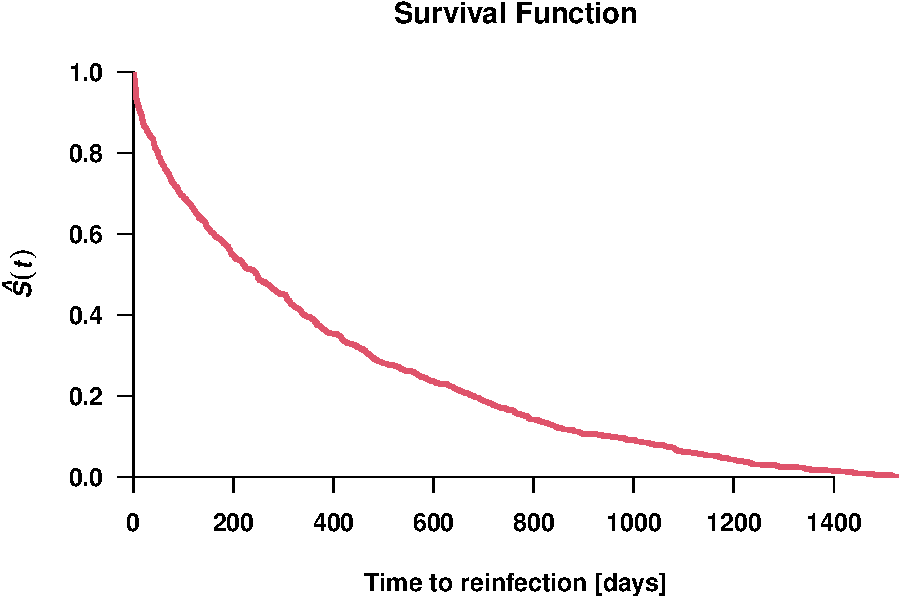
\includegraphics{practical_files/figure-latex/unnamed-chunk-6-1.pdf}

\begin{Shaded}
\begin{Highlighting}[]
\NormalTok{s1.CondomUse }\OtherTok{\textless{}{-}} \FunctionTok{with}\NormalTok{(std\_data, }\FunctionTok{Surv}\NormalTok{(TimeUntilReinf, cens) }\SpecialCharTok{\textasciitilde{}}\NormalTok{ CondomUse)}
\NormalTok{s1fit.CondomUse }\OtherTok{\textless{}{-}} \FunctionTok{survfit}\NormalTok{(s1.CondomUse)}
\FunctionTok{par}\NormalTok{(}\AttributeTok{font =} \DecValTok{2}\NormalTok{, }\AttributeTok{font.axis =} \DecValTok{2}\NormalTok{, }\AttributeTok{font.lab =} \DecValTok{2}\NormalTok{, }\AttributeTok{las =} \DecValTok{1}\NormalTok{, }\AttributeTok{mar =} \FunctionTok{c}\NormalTok{(}\DecValTok{5}\NormalTok{, }\DecValTok{5}\NormalTok{, }\DecValTok{4}\NormalTok{, }\DecValTok{2}\NormalTok{))}
\FunctionTok{plot}\NormalTok{(s1fit.CondomUse, }\AttributeTok{col =} \FunctionTok{c}\NormalTok{(}\DecValTok{1}\NormalTok{,}\DecValTok{2}\NormalTok{,}\DecValTok{3}\NormalTok{), }\AttributeTok{xlab =} \StringTok{"Time to reinfection [days]"}\NormalTok{,}
     \AttributeTok{ylab =} \FunctionTok{expression}\NormalTok{(}\FunctionTok{bolditalic}\NormalTok{(}\FunctionTok{hat}\NormalTok{(S)(t))),}
     \AttributeTok{yaxs =} \StringTok{"i"}\NormalTok{, }\AttributeTok{xaxs =} \StringTok{"i"}\NormalTok{, }\AttributeTok{bty =} \StringTok{"n"}\NormalTok{, }\AttributeTok{lty =} \FunctionTok{c}\NormalTok{(}\DecValTok{1}\NormalTok{,}\DecValTok{2}\NormalTok{,}\DecValTok{3}\NormalTok{), }\AttributeTok{lwd =} \FunctionTok{rep}\NormalTok{(}\DecValTok{3}\NormalTok{, }\AttributeTok{length.out =} \DecValTok{3}\NormalTok{),}
     \AttributeTok{conf.int =}\NormalTok{ F)}
\FunctionTok{legend}\NormalTok{(}\StringTok{"topright"}\NormalTok{, }\AttributeTok{legend =} \FunctionTok{levels}\NormalTok{(std\_data}\SpecialCharTok{$}\NormalTok{CondomUse), }\AttributeTok{title =} \StringTok{"Condom Use"}\NormalTok{,}
       \AttributeTok{bty =} \StringTok{"n"}\NormalTok{, }\AttributeTok{col =} \FunctionTok{c}\NormalTok{(}\DecValTok{1}\NormalTok{,}\DecValTok{2}\NormalTok{,}\DecValTok{3}\NormalTok{), }\AttributeTok{lty =} \FunctionTok{c}\NormalTok{(}\DecValTok{1}\NormalTok{,}\DecValTok{2}\NormalTok{,}\DecValTok{3}\NormalTok{), }\AttributeTok{lwd =} \FunctionTok{rep}\NormalTok{(}\DecValTok{3}\NormalTok{, }\AttributeTok{length.out =} \DecValTok{3}\NormalTok{))}
\FunctionTok{title}\NormalTok{(}\StringTok{"Survival Function as Function of Condom Use"}\NormalTok{)}
\end{Highlighting}
\end{Shaded}

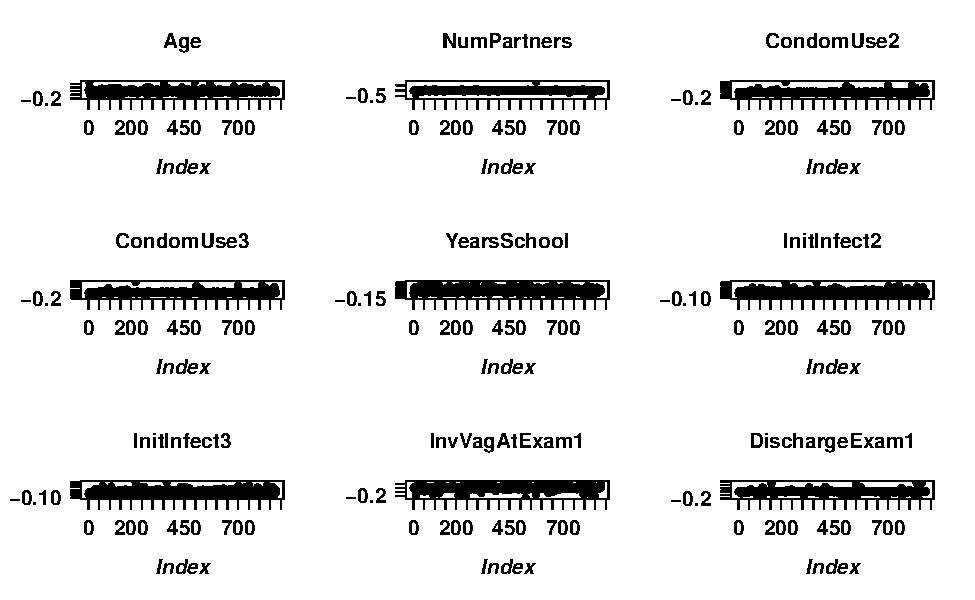
\includegraphics{practical_files/figure-latex/unnamed-chunk-7-1.pdf}

\begin{Shaded}
\begin{Highlighting}[]
\NormalTok{s1.Ethnicity }\OtherTok{\textless{}{-}} \FunctionTok{with}\NormalTok{(std\_data, }\FunctionTok{Surv}\NormalTok{(TimeUntilReinf, cens) }\SpecialCharTok{\textasciitilde{}}\NormalTok{ Ethnicity)}
\NormalTok{s1fit.Ethnicity }\OtherTok{\textless{}{-}} \FunctionTok{survfit}\NormalTok{(s1.Ethnicity)}
\FunctionTok{par}\NormalTok{(}\AttributeTok{font =} \DecValTok{2}\NormalTok{, }\AttributeTok{font.axis =} \DecValTok{2}\NormalTok{, }\AttributeTok{font.lab =} \DecValTok{2}\NormalTok{, }\AttributeTok{las =} \DecValTok{1}\NormalTok{, }\AttributeTok{mar =} \FunctionTok{c}\NormalTok{(}\DecValTok{5}\NormalTok{, }\DecValTok{5}\NormalTok{, }\DecValTok{4}\NormalTok{, }\DecValTok{2}\NormalTok{))}
\FunctionTok{plot}\NormalTok{(s1fit.Ethnicity, }\AttributeTok{col =} \FunctionTok{c}\NormalTok{(}\DecValTok{1}\NormalTok{,}\DecValTok{2}\NormalTok{), }\AttributeTok{xlab =} \StringTok{"Time to reinfection [days]"}\NormalTok{,}
     \AttributeTok{ylab =} \FunctionTok{expression}\NormalTok{(}\FunctionTok{bolditalic}\NormalTok{(}\FunctionTok{hat}\NormalTok{(S)(t))),}
     \AttributeTok{yaxs =} \StringTok{"i"}\NormalTok{, }\AttributeTok{xaxs =} \StringTok{"i"}\NormalTok{, }\AttributeTok{bty =} \StringTok{"n"}\NormalTok{, }\AttributeTok{lty =} \FunctionTok{c}\NormalTok{(}\DecValTok{1}\NormalTok{,}\DecValTok{2}\NormalTok{), }\AttributeTok{lwd =} \FunctionTok{rep}\NormalTok{(}\DecValTok{3}\NormalTok{, }\AttributeTok{length.out =} \DecValTok{2}\NormalTok{),}
     \AttributeTok{conf.int =}\NormalTok{ F)}
\FunctionTok{legend}\NormalTok{(}\StringTok{"topright"}\NormalTok{, }\AttributeTok{legend =} \FunctionTok{levels}\NormalTok{(std\_data}\SpecialCharTok{$}\NormalTok{Ethnicity), }\AttributeTok{title =} \StringTok{"Ethnicity"}\NormalTok{,}
       \AttributeTok{bty =} \StringTok{"n"}\NormalTok{, }\AttributeTok{col =} \FunctionTok{c}\NormalTok{(}\DecValTok{1}\NormalTok{,}\DecValTok{2}\NormalTok{), }\AttributeTok{lty =} \FunctionTok{c}\NormalTok{(}\DecValTok{1}\NormalTok{,}\DecValTok{2}\NormalTok{), }\AttributeTok{lwd =} \FunctionTok{rep}\NormalTok{(}\DecValTok{3}\NormalTok{, }\AttributeTok{length.out =} \DecValTok{2}\NormalTok{))}
\FunctionTok{title}\NormalTok{(}\StringTok{"Survival Function as Function of Ethnicity"}\NormalTok{)}
\end{Highlighting}
\end{Shaded}

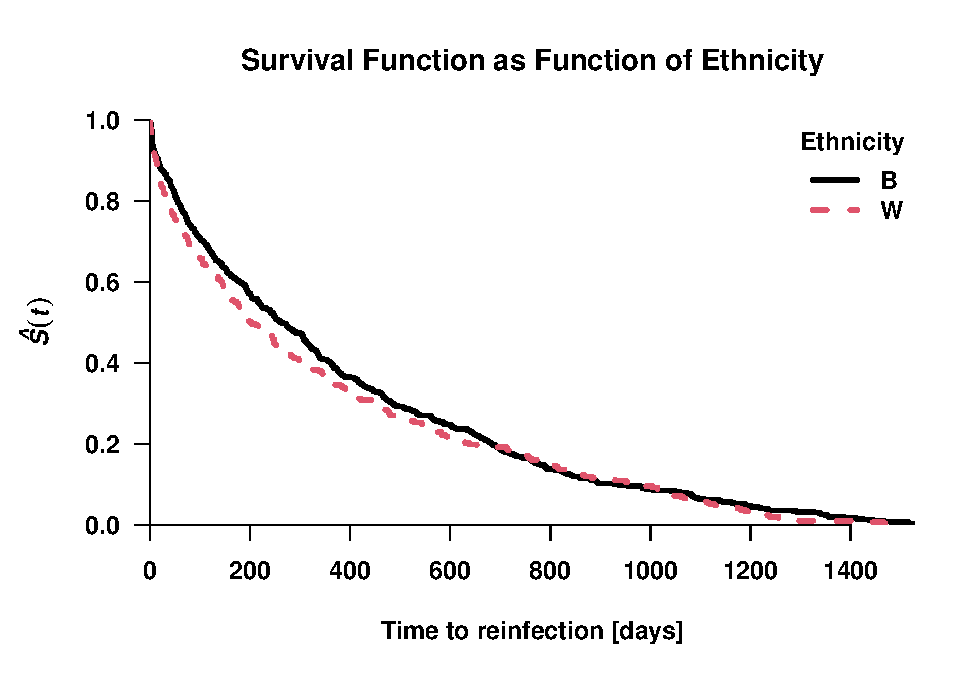
\includegraphics{practical_files/figure-latex/unnamed-chunk-8-1.pdf}

\begin{Shaded}
\begin{Highlighting}[]
\NormalTok{s1.SignDischarge }\OtherTok{\textless{}{-}} \FunctionTok{with}\NormalTok{(std\_data, }\FunctionTok{Surv}\NormalTok{(TimeUntilReinf, cens) }\SpecialCharTok{\textasciitilde{}}\NormalTok{ SignDischarge)}
\NormalTok{s1fit.SignDischarge }\OtherTok{\textless{}{-}} \FunctionTok{survfit}\NormalTok{(s1.SignDischarge)}
\FunctionTok{par}\NormalTok{(}\AttributeTok{font =} \DecValTok{2}\NormalTok{, }\AttributeTok{font.axis =} \DecValTok{2}\NormalTok{, }\AttributeTok{font.lab =} \DecValTok{2}\NormalTok{, }\AttributeTok{las =} \DecValTok{1}\NormalTok{, }\AttributeTok{mar =} \FunctionTok{c}\NormalTok{(}\DecValTok{5}\NormalTok{, }\DecValTok{5}\NormalTok{, }\DecValTok{4}\NormalTok{, }\DecValTok{2}\NormalTok{))}
\FunctionTok{plot}\NormalTok{(s1fit.SignDischarge, }\AttributeTok{col =} \FunctionTok{c}\NormalTok{(}\DecValTok{1}\NormalTok{,}\DecValTok{2}\NormalTok{), }\AttributeTok{xlab =} \StringTok{"Time to reinfection [days]"}\NormalTok{,}
     \AttributeTok{ylab =} \FunctionTok{expression}\NormalTok{(}\FunctionTok{bolditalic}\NormalTok{(}\FunctionTok{hat}\NormalTok{(S)(t))),}
     \AttributeTok{yaxs =} \StringTok{"i"}\NormalTok{, }\AttributeTok{xaxs =} \StringTok{"i"}\NormalTok{, }\AttributeTok{bty =} \StringTok{"n"}\NormalTok{, }\AttributeTok{lty =} \FunctionTok{c}\NormalTok{(}\DecValTok{1}\NormalTok{,}\DecValTok{2}\NormalTok{), }\AttributeTok{lwd =} \FunctionTok{rep}\NormalTok{(}\DecValTok{3}\NormalTok{, }\AttributeTok{length.out =} \DecValTok{2}\NormalTok{),}
     \AttributeTok{conf.int =}\NormalTok{ F)}
\FunctionTok{legend}\NormalTok{(}\StringTok{"topright"}\NormalTok{, }\AttributeTok{legend =} \FunctionTok{levels}\NormalTok{(std\_data}\SpecialCharTok{$}\NormalTok{SignDischarge), }\AttributeTok{title =} \StringTok{"Sign of Discharge"}\NormalTok{,}
       \AttributeTok{bty =} \StringTok{"n"}\NormalTok{, }\AttributeTok{col =} \FunctionTok{c}\NormalTok{(}\DecValTok{1}\NormalTok{,}\DecValTok{2}\NormalTok{), }\AttributeTok{lty =} \FunctionTok{c}\NormalTok{(}\DecValTok{1}\NormalTok{,}\DecValTok{2}\NormalTok{), }\AttributeTok{lwd =} \FunctionTok{rep}\NormalTok{(}\DecValTok{3}\NormalTok{, }\AttributeTok{length.out =} \DecValTok{2}\NormalTok{))}
\FunctionTok{title}\NormalTok{(}\StringTok{"Survival Function as Function of Sign of Discharge"}\NormalTok{)}
\end{Highlighting}
\end{Shaded}

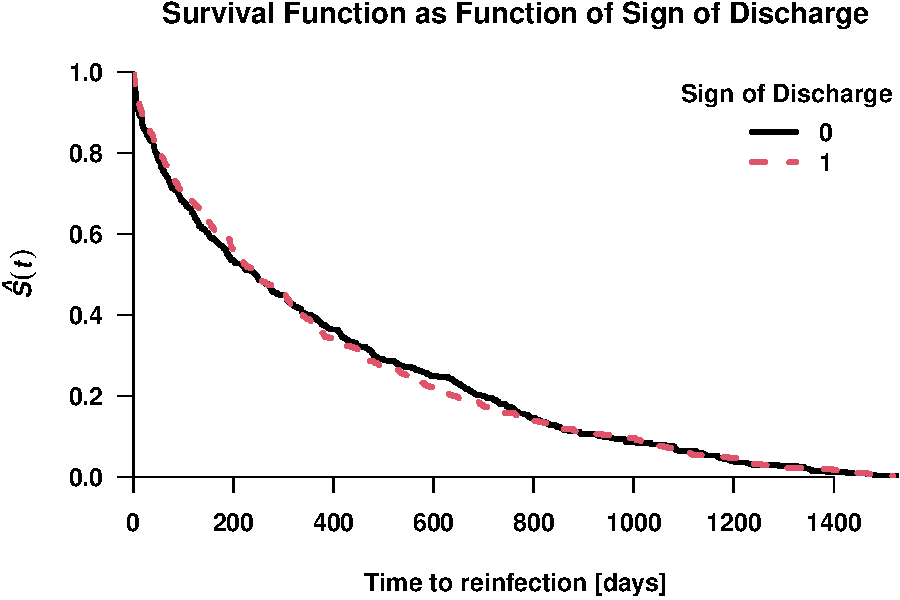
\includegraphics{practical_files/figure-latex/unnamed-chunk-9-1.pdf}

\begin{Shaded}
\begin{Highlighting}[]
\NormalTok{s1.NumPartners }\OtherTok{\textless{}{-}} \FunctionTok{with}\NormalTok{(std\_data, }\FunctionTok{Surv}\NormalTok{(TimeUntilReinf, cens) }\SpecialCharTok{\textasciitilde{}}\NormalTok{ NumPartners)}
\NormalTok{s1fit.NumPartners }\OtherTok{\textless{}{-}} \FunctionTok{survfit}\NormalTok{(s1.NumPartners)}
\FunctionTok{par}\NormalTok{(}\AttributeTok{font =} \DecValTok{2}\NormalTok{, }\AttributeTok{font.axis =} \DecValTok{2}\NormalTok{, }\AttributeTok{font.lab =} \DecValTok{2}\NormalTok{, }\AttributeTok{las =} \DecValTok{1}\NormalTok{, }\AttributeTok{mar =} \FunctionTok{c}\NormalTok{(}\DecValTok{5}\NormalTok{, }\DecValTok{5}\NormalTok{, }\DecValTok{4}\NormalTok{, }\DecValTok{2}\NormalTok{))}
\FunctionTok{plot}\NormalTok{(s1fit.NumPartners, }\AttributeTok{col =} \FunctionTok{c}\NormalTok{(}\DecValTok{1}\NormalTok{,}\DecValTok{2}\NormalTok{,}\DecValTok{3}\NormalTok{,}\DecValTok{4}\NormalTok{,}\DecValTok{5}\NormalTok{,}\DecValTok{6}\NormalTok{,}\DecValTok{7}\NormalTok{,}\DecValTok{8}\NormalTok{,}\DecValTok{9}\NormalTok{), }\AttributeTok{xlab =} \StringTok{"Time to reinfection [days]"}\NormalTok{,}
     \AttributeTok{ylab =} \FunctionTok{expression}\NormalTok{(}\FunctionTok{bolditalic}\NormalTok{(}\FunctionTok{hat}\NormalTok{(S)(t))),}
     \AttributeTok{yaxs =} \StringTok{"i"}\NormalTok{, }\AttributeTok{xaxs =} \StringTok{"i"}\NormalTok{, }\AttributeTok{bty =} \StringTok{"n"}\NormalTok{, }\AttributeTok{lty =} \FunctionTok{c}\NormalTok{(}\DecValTok{1}\NormalTok{,}\DecValTok{2}\NormalTok{,}\DecValTok{3}\NormalTok{,}\DecValTok{4}\NormalTok{,}\DecValTok{5}\NormalTok{,}\DecValTok{6}\NormalTok{,}\DecValTok{7}\NormalTok{,}\DecValTok{8}\NormalTok{,}\DecValTok{9}\NormalTok{), }\AttributeTok{lwd =} \FunctionTok{rep}\NormalTok{(}\DecValTok{3}\NormalTok{, }\AttributeTok{length.out =} \DecValTok{9}\NormalTok{),}
     \AttributeTok{conf.int =}\NormalTok{ F)}
\FunctionTok{legend}\NormalTok{(}\StringTok{"topright"}\NormalTok{, }\AttributeTok{legend =} \FunctionTok{levels}\NormalTok{(}\FunctionTok{as.factor}\NormalTok{(std\_data}\SpecialCharTok{$}\NormalTok{NumPartners)), }\AttributeTok{title =} \StringTok{"Number of Partners"}\NormalTok{,}
       \AttributeTok{bty =} \StringTok{"n"}\NormalTok{, }\AttributeTok{col =} \FunctionTok{c}\NormalTok{(}\DecValTok{1}\NormalTok{,}\DecValTok{2}\NormalTok{,}\DecValTok{3}\NormalTok{,}\DecValTok{4}\NormalTok{,}\DecValTok{5}\NormalTok{,}\DecValTok{6}\NormalTok{,}\DecValTok{7}\NormalTok{,}\DecValTok{8}\NormalTok{,}\DecValTok{9}\NormalTok{), }\AttributeTok{lty =} \FunctionTok{c}\NormalTok{(}\DecValTok{1}\NormalTok{,}\DecValTok{2}\NormalTok{,}\DecValTok{3}\NormalTok{,}\DecValTok{4}\NormalTok{,}\DecValTok{5}\NormalTok{,}\DecValTok{6}\NormalTok{,}\DecValTok{7}\NormalTok{,}\DecValTok{8}\NormalTok{,}\DecValTok{9}\NormalTok{), }\AttributeTok{lwd =} \FunctionTok{rep}\NormalTok{(}\DecValTok{3}\NormalTok{, }\AttributeTok{length.out =} \DecValTok{9}\NormalTok{))}
\FunctionTok{title}\NormalTok{(}\StringTok{"Survival Function as Function of Number of Partners"}\NormalTok{)}
\end{Highlighting}
\end{Shaded}

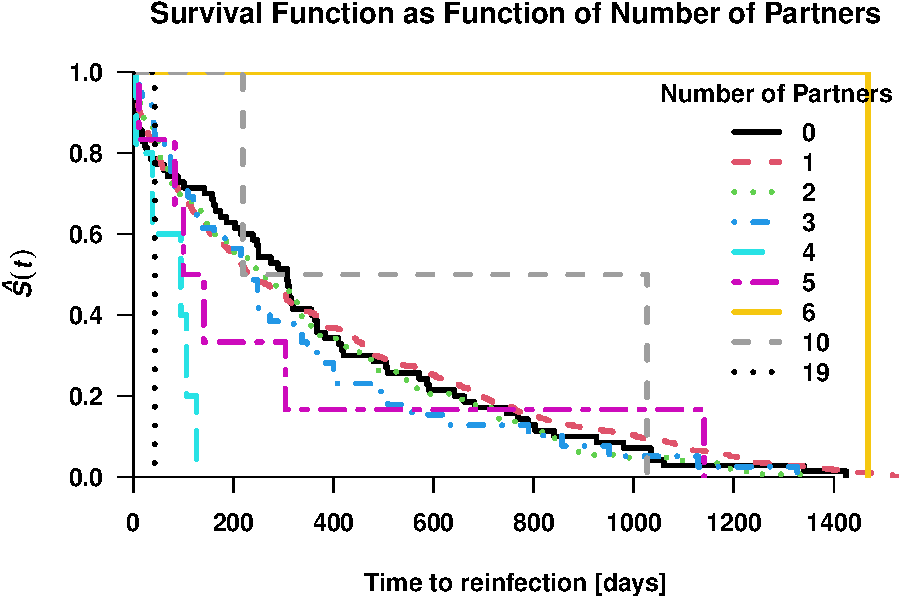
\includegraphics{practical_files/figure-latex/unnamed-chunk-10-1.pdf}

The median survival time is 247 days, as can be seen below.

\begin{Shaded}
\begin{Highlighting}[]
\NormalTok{s1fit}
\end{Highlighting}
\end{Shaded}

\begin{verbatim}
#> Call: survfit(formula = s1)
#> 
#>       n  events  median 0.95LCL 0.95UCL 
#>     877     877     247     216     277
\end{verbatim}

Comparison of survival functions by means of nonparametric tests, such as the logrank test. The curve on ethnicity could be interesting to test (the survivals cross though!)

Below, logrank test for all curves plotted above are done.

\begin{Shaded}
\begin{Highlighting}[]
\FunctionTok{FHtestrcc}\NormalTok{(s1.CondomUse)}
\end{Highlighting}
\end{Shaded}

\begin{verbatim}
#> 
#>  K-sample test for right-censored data
#> 
#> Parameters: rho=0, lambda=0
#> Distribution: counting process approach
#> 
#> Data: Surv(TimeUntilReinf, cens) by CondomUse
#> 
#>               N Observed Expected    O-E (O-E)^2/E (O-E)^2/V
#> CondomUse=1  54       54     51.8   2.16    0.0902    0.0968
#> CondomUse=2 511      511    457.3  53.66    6.2948   13.4467
#> CondomUse=3 312      312    367.8 -55.82    8.4704   14.8506
#> 
#> Chisq= 15.1 on 2 degrees of freedom, p-value= 0.000514
#> Alternative hypothesis: survival functions not equal
\end{verbatim}

\begin{Shaded}
\begin{Highlighting}[]
\FunctionTok{FHtestrcc}\NormalTok{(s1.Ethnicity)}
\end{Highlighting}
\end{Shaded}

\begin{verbatim}
#> 
#>  Two-sample test for right-censored data
#> 
#> Parameters: rho=0, lambda=0
#> Distribution: counting process approach
#> 
#> Data: Surv(TimeUntilReinf, cens) by Ethnicity
#> 
#>               N Observed Expected   O-E (O-E)^2/E (O-E)^2/V
#> Ethnicity=B 585      585      603 -18.3     0.555       1.8
#> Ethnicity=W 292      292      274  18.3     1.224       1.8
#> 
#> Statistic Z= 1.3, p-value= 0.18
#> Alternative hypothesis: survival functions not equal
\end{verbatim}

\begin{Shaded}
\begin{Highlighting}[]
\FunctionTok{FHtestrcc}\NormalTok{(s1.SignDischarge)}
\end{Highlighting}
\end{Shaded}

\begin{verbatim}
#> 
#>  Two-sample test for right-censored data
#> 
#> Parameters: rho=0, lambda=0
#> Distribution: counting process approach
#> 
#> Data: Surv(TimeUntilReinf, cens) by SignDischarge
#> 
#>                   N Observed Expected    O-E (O-E)^2/E (O-E)^2/V
#> SignDischarge=0 472      472      472 -0.461  0.000450   0.00098
#> SignDischarge=1 405      405      405  0.461  0.000525   0.00098
#> 
#> Statistic Z= 0, p-value= 0.975
#> Alternative hypothesis: survival functions not equal
\end{verbatim}

\begin{Shaded}
\begin{Highlighting}[]
\FunctionTok{FHtestrcc}\NormalTok{(s1.NumPartners)}
\end{Highlighting}
\end{Shaded}

\begin{verbatim}
#> 
#>  Trend FH test for right-censored data
#> 
#> Parameters: rho=0, lambda=0
#> Distribution: counting process approach
#> 
#> Data: Surv(TimeUntilReinf, cens) by NumPartners
#> 
#>                  N Observed Expected     O-E
#> NumPartners=0   70       70   67.796   2.204
#> NumPartners=1  607      607  626.599 -19.599
#> NumPartners=2  146      146  134.200  11.800
#> NumPartners=3   39       39   33.838   5.162
#> NumPartners=4    5        5    1.417   3.583
#> NumPartners=5    6        6    4.944   1.056
#> NumPartners=6    1        1    4.895  -3.895
#> NumPartners=10   2        2    3.104  -1.104
#> NumPartners=19   1        1    0.206   0.794
#> 
#> Statistic Z= 0.7, p-value= 0.488
#> Alternative hypothesis: survival functions not equal
\end{verbatim}

\hypertarget{fit-of-a-parametric-survival-model}{%
\section{Fit of a parametric survival model}\label{fit-of-a-parametric-survival-model}}

Fit a Weibull, log-logistic or lognormal model. Justify the theoretical choice we are taking!!

\begin{Shaded}
\begin{Highlighting}[]
\CommentTok{\# I am testing all three below, since I am not sure which will be better.}

\CommentTok{\# Below we have the null models. }
\NormalTok{s2 }\OtherTok{\textless{}{-}} \FunctionTok{with}\NormalTok{(std\_data, }\FunctionTok{Surv}\NormalTok{(TimeUntilReinf, cens))}
\NormalTok{loglo }\OtherTok{\textless{}{-}} \FunctionTok{survreg}\NormalTok{(s2 }\SpecialCharTok{\textasciitilde{}} \DecValTok{1}\NormalTok{, }\AttributeTok{dist =} \StringTok{"loglo"}\NormalTok{)  }
\FunctionTok{summary}\NormalTok{(loglo)}
\end{Highlighting}
\end{Shaded}

\begin{verbatim}
#> 
#> Call:
#> survreg(formula = s2 ~ 1, dist = "loglo")
#>               Value Std. Error     z       p
#> (Intercept)  5.2914     0.0532 99.52 < 2e-16
#> Log(scale)  -0.0995     0.0283 -3.51 0.00045
#> 
#> Scale= 0.905 
#> 
#> Log logistic distribution
#> Loglik(model)= -6139.9   Loglik(intercept only)= -6139.9
#> Number of Newton-Raphson Iterations: 6 
#> n= 877
\end{verbatim}

\begin{Shaded}
\begin{Highlighting}[]
\NormalTok{weibull }\OtherTok{\textless{}{-}} \FunctionTok{survreg}\NormalTok{(s2 }\SpecialCharTok{\textasciitilde{}} \DecValTok{1}\NormalTok{)}
\FunctionTok{summary}\NormalTok{(weibull)}
\end{Highlighting}
\end{Shaded}

\begin{verbatim}
#> 
#> Call:
#> survreg(formula = s2 ~ 1)
#>              Value Std. Error      z       p
#> (Intercept) 5.8289     0.0423 137.94 < 2e-16
#> Log(scale)  0.1762     0.0277   6.37 1.9e-10
#> 
#> Scale= 1.19 
#> 
#> Weibull distribution
#> Loglik(model)= -6040.1   Loglik(intercept only)= -6040.1
#> Number of Newton-Raphson Iterations: 7 
#> n= 877
\end{verbatim}

\begin{Shaded}
\begin{Highlighting}[]
\NormalTok{lognormal }\OtherTok{\textless{}{-}} \FunctionTok{survreg}\NormalTok{(s2 }\SpecialCharTok{\textasciitilde{}} \DecValTok{1}\NormalTok{, }\AttributeTok{dist =} \StringTok{"lognormal"}\NormalTok{)}
\FunctionTok{summary}\NormalTok{(lognormal)}
\end{Highlighting}
\end{Shaded}

\begin{verbatim}
#> 
#> Call:
#> survreg(formula = s2 ~ 1, dist = "lognormal")
#>              Value Std. Error    z      p
#> (Intercept) 5.0988     0.0553 92.2 <2e-16
#> Log(scale)  0.4934     0.0239 20.7 <2e-16
#> 
#> Scale= 1.64 
#> 
#> Log Normal distribution
#> Loglik(model)= -6148.8   Loglik(intercept only)= -6148.8
#> Number of Newton-Raphson Iterations: 5 
#> n= 877
\end{verbatim}

\begin{Shaded}
\begin{Highlighting}[]
\CommentTok{\# Below we add some covariates to the models. INCLUDE ALL OF THEM PERHAPS! (OR }\AlertTok{TEST}\CommentTok{ WITH DIFFERENT ONES!)}
\CommentTok{\# First we add Ethnicity  e.g.}
\NormalTok{loglo.Ethnicity }\OtherTok{\textless{}{-}} \FunctionTok{survreg}\NormalTok{(s2 }\SpecialCharTok{\textasciitilde{}}\NormalTok{ Ethnicity, }\AttributeTok{dist =} \StringTok{"loglo"}\NormalTok{, }\AttributeTok{data =}\NormalTok{ std\_data)  }
\FunctionTok{summary}\NormalTok{(loglo.Ethnicity)}
\end{Highlighting}
\end{Shaded}

\begin{verbatim}
#> 
#> Call:
#> survreg(formula = s2 ~ Ethnicity, data = std_data, dist = "loglo")
#>               Value Std. Error     z       p
#> (Intercept)  5.3566     0.0642 83.38 < 2e-16
#> EthnicityW  -0.2016     0.1133 -1.78 0.07520
#> Log(scale)  -0.1013     0.0283 -3.58 0.00035
#> 
#> Scale= 0.904 
#> 
#> Log logistic distribution
#> Loglik(model)= -6138.4   Loglik(intercept only)= -6139.9
#>  Chisq= 3.17 on 1 degrees of freedom, p= 0.075 
#> Number of Newton-Raphson Iterations: 4 
#> n= 877
\end{verbatim}

\begin{Shaded}
\begin{Highlighting}[]
\NormalTok{weibull.Ethnicity }\OtherTok{\textless{}{-}} \FunctionTok{survreg}\NormalTok{(s2 }\SpecialCharTok{\textasciitilde{}}\NormalTok{ Ethnicity, }\AttributeTok{data =}\NormalTok{ std\_data)}
\FunctionTok{summary}\NormalTok{(weibull.Ethnicity)}
\end{Highlighting}
\end{Shaded}

\begin{verbatim}
#> 
#> Call:
#> survreg(formula = s2 ~ Ethnicity, data = std_data)
#>               Value Std. Error      z      p
#> (Intercept)  5.8606     0.0508 115.41 <2e-16
#> EthnicityW  -0.0973     0.0855  -1.14   0.25
#> Log(scale)   0.1759     0.0276   6.36  2e-10
#> 
#> Scale= 1.19 
#> 
#> Weibull distribution
#> Loglik(model)= -6039.4   Loglik(intercept only)= -6040.1
#>  Chisq= 1.29 on 1 degrees of freedom, p= 0.26 
#> Number of Newton-Raphson Iterations: 6 
#> n= 877
\end{verbatim}

\begin{Shaded}
\begin{Highlighting}[]
\NormalTok{lognormal.Ethnicity }\OtherTok{\textless{}{-}} \FunctionTok{survreg}\NormalTok{(s2 }\SpecialCharTok{\textasciitilde{}}\NormalTok{ Ethnicity, }\AttributeTok{dist =} \StringTok{"lognormal"}\NormalTok{, }\AttributeTok{data =}\NormalTok{ std\_data)}
\FunctionTok{summary}\NormalTok{(lognormal.Ethnicity)}
\end{Highlighting}
\end{Shaded}

\begin{verbatim}
#> 
#> Call:
#> survreg(formula = s2 ~ Ethnicity, data = std_data, dist = "lognormal")
#>               Value Std. Error     z      p
#> (Intercept)  5.1681     0.0676 76.45 <2e-16
#> EthnicityW  -0.2080     0.1171 -1.78  0.076
#> Log(scale)   0.4916     0.0239 20.59 <2e-16
#> 
#> Scale= 1.63 
#> 
#> Log Normal distribution
#> Loglik(model)= -6147.2   Loglik(intercept only)= -6148.8
#>  Chisq= 3.15 on 1 degrees of freedom, p= 0.076 
#> Number of Newton-Raphson Iterations: 2 
#> n= 877
\end{verbatim}

\begin{Shaded}
\begin{Highlighting}[]
\NormalTok{loglo.full }\OtherTok{\textless{}{-}} \FunctionTok{survreg}\NormalTok{(s2 }\SpecialCharTok{\textasciitilde{}}\NormalTok{ Ethnicity }\SpecialCharTok{+}\NormalTok{ Age }\SpecialCharTok{+}\NormalTok{ NumPartners }\SpecialCharTok{+}\NormalTok{ CondomUse }\SpecialCharTok{+}\NormalTok{ YearsSchool }\SpecialCharTok{+}\NormalTok{ SignDischarge, }\AttributeTok{data =}\NormalTok{ std\_data, }\AttributeTok{dist =} \StringTok{"loglo"}\NormalTok{)}
\FunctionTok{summary}\NormalTok{(loglo.full)}
\end{Highlighting}
\end{Shaded}

\begin{verbatim}
#> 
#> Call:
#> survreg(formula = s2 ~ Ethnicity + Age + NumPartners + CondomUse + 
#>     YearsSchool + SignDischarge, data = std_data, dist = "loglo")
#>                   Value Std. Error     z      p
#> (Intercept)     4.43176    0.43979 10.08 <2e-16
#> EthnicityW     -0.20875    0.11403 -1.83 0.0672
#> Age            -0.00381    0.01125 -0.34 0.7346
#> NumPartners    -0.01960    0.04942 -0.40 0.6917
#> CondomUse2      0.34934    0.23892  1.46 0.1437
#> CondomUse3      0.67345    0.24619  2.74 0.0062
#> YearsSchool     0.04901    0.03487  1.41 0.1599
#> SignDischarge1  0.05863    0.10562  0.56 0.5788
#> Log(scale)     -0.11108    0.02836 -3.92  9e-05
#> 
#> Scale= 0.895 
#> 
#> Log logistic distribution
#> Loglik(model)= -6130.8   Loglik(intercept only)= -6139.9
#>  Chisq= 18.39 on 7 degrees of freedom, p= 0.01 
#> Number of Newton-Raphson Iterations: 4 
#> n= 877
\end{verbatim}

\begin{Shaded}
\begin{Highlighting}[]
\NormalTok{loglo.pred }\OtherTok{\textless{}{-}} \FunctionTok{predict}\NormalTok{(loglo.full, }\AttributeTok{type =} \StringTok{"linear"}\NormalTok{)}
\NormalTok{resids.loglo }\OtherTok{\textless{}{-}}\NormalTok{ (}\FunctionTok{log}\NormalTok{(std\_data}\SpecialCharTok{$}\NormalTok{TimeUntilReinf) }\SpecialCharTok{{-}}\NormalTok{ loglo.pred) }\SpecialCharTok{/}\NormalTok{ loglo.full}\SpecialCharTok{$}\NormalTok{scale}

\NormalTok{weibull.full }\OtherTok{\textless{}{-}} \FunctionTok{update}\NormalTok{(loglo.full, }\AttributeTok{dist =} \StringTok{"weibull"}\NormalTok{)}
\FunctionTok{summary}\NormalTok{(weibull.full)}
\end{Highlighting}
\end{Shaded}

\begin{verbatim}
#> 
#> Call:
#> survreg(formula = s2 ~ Ethnicity + Age + NumPartners + CondomUse + 
#>     YearsSchool + SignDischarge, data = std_data, dist = "weibull")
#>                    Value Std. Error     z       p
#> (Intercept)     5.310720   0.328119 16.19 < 2e-16
#> EthnicityW     -0.110680   0.085688 -1.29    0.20
#> Age            -0.001799   0.008523 -0.21    0.83
#> NumPartners    -0.010662   0.040943 -0.26    0.79
#> CondomUse2      0.009896   0.169834  0.06    0.95
#> CondomUse3      0.285457   0.175474  1.63    0.10
#> YearsSchool     0.043070   0.026987  1.60    0.11
#> SignDischarge1 -0.000572   0.080803 -0.01    0.99
#> Log(scale)      0.166530   0.027666  6.02 1.8e-09
#> 
#> Scale= 1.18 
#> 
#> Weibull distribution
#> Loglik(model)= -6031.9   Loglik(intercept only)= -6040.1
#>  Chisq= 16.29 on 7 degrees of freedom, p= 0.023 
#> Number of Newton-Raphson Iterations: 6 
#> n= 877
\end{verbatim}

\begin{Shaded}
\begin{Highlighting}[]
\NormalTok{weibull.pred }\OtherTok{\textless{}{-}} \FunctionTok{predict}\NormalTok{(weibull.full, }\AttributeTok{type =} \StringTok{"linear"}\NormalTok{)}
\NormalTok{resids.weibull }\OtherTok{\textless{}{-}}\NormalTok{ (}\FunctionTok{log}\NormalTok{(std\_data}\SpecialCharTok{$}\NormalTok{TimeUntilReinf) }\SpecialCharTok{{-}}\NormalTok{ weibull.pred) }\SpecialCharTok{/}\NormalTok{ weibull.full}\SpecialCharTok{$}\NormalTok{scale}

\NormalTok{lognormal.full }\OtherTok{\textless{}{-}} \FunctionTok{update}\NormalTok{(loglo.full, }\AttributeTok{dist =} \StringTok{"lognormal"}\NormalTok{)}
\FunctionTok{summary}\NormalTok{(lognormal.full)}
\end{Highlighting}
\end{Shaded}

\begin{verbatim}
#> 
#> Call:
#> survreg(formula = s2 ~ Ethnicity + Age + NumPartners + CondomUse + 
#>     YearsSchool + SignDischarge, data = std_data, dist = "lognormal")
#>                  Value Std. Error     z      p
#> (Intercept)     4.1690     0.4468  9.33 <2e-16
#> EthnicityW     -0.2198     0.1177 -1.87 0.0620
#> Age            -0.0018     0.0115 -0.16 0.8763
#> NumPartners     0.0172     0.0536  0.32 0.7484
#> CondomUse2      0.3114     0.2331  1.34 0.1815
#> CondomUse3      0.6232     0.2412  2.58 0.0098
#> YearsSchool     0.0510     0.0359  1.42 0.1554
#> SignDischarge1  0.0708     0.1107  0.64 0.5224
#> Log(scale)      0.4841     0.0239 20.27 <2e-16
#> 
#> Scale= 1.62 
#> 
#> Log Normal distribution
#> Loglik(model)= -6140.6   Loglik(intercept only)= -6148.8
#>  Chisq= 16.34 on 7 degrees of freedom, p= 0.022 
#> Number of Newton-Raphson Iterations: 3 
#> n= 877
\end{verbatim}

\begin{Shaded}
\begin{Highlighting}[]
\NormalTok{lognormal.pred }\OtherTok{\textless{}{-}} \FunctionTok{predict}\NormalTok{(lognormal.full, }\AttributeTok{type =} \StringTok{"linear"}\NormalTok{)}
\NormalTok{resids.logno }\OtherTok{\textless{}{-}}\NormalTok{ (}\FunctionTok{log}\NormalTok{(std\_data}\SpecialCharTok{$}\NormalTok{TimeUntilReinf) }\SpecialCharTok{{-}}\NormalTok{ lognormal.pred) }\SpecialCharTok{/}\NormalTok{ lognormal.full}\SpecialCharTok{$}\NormalTok{scale}

\CommentTok{\# Model checking (using residuals etc, as done in lab 6).}
\CommentTok{\# Log{-}logistic}
\FunctionTok{par}\NormalTok{(}\AttributeTok{font =} \DecValTok{2}\NormalTok{, }\AttributeTok{font.axis =} \DecValTok{2}\NormalTok{, }\AttributeTok{font.lab =} \DecValTok{2}\NormalTok{, }\AttributeTok{las =} \DecValTok{1}\NormalTok{, }\AttributeTok{mar =} \FunctionTok{c}\NormalTok{(}\DecValTok{5}\NormalTok{, }\DecValTok{5}\NormalTok{, }\DecValTok{4}\NormalTok{, }\DecValTok{2}\NormalTok{))}
\FunctionTok{plot}\NormalTok{(}\FunctionTok{survfit}\NormalTok{(}\FunctionTok{Surv}\NormalTok{(resids.loglo, std\_data}\SpecialCharTok{$}\NormalTok{cens) }\SpecialCharTok{\textasciitilde{}} \DecValTok{1}\NormalTok{), }\AttributeTok{col =} \FunctionTok{c}\NormalTok{(}\DecValTok{1}\NormalTok{,}\DecValTok{2}\NormalTok{,}\DecValTok{2}\NormalTok{), }\AttributeTok{xlab =} \StringTok{"Residuals"}\NormalTok{,}
     \AttributeTok{ylab =} \FunctionTok{expression}\NormalTok{(}\FunctionTok{bolditalic}\NormalTok{(}\FunctionTok{hat}\NormalTok{(S)(t))),}
     \AttributeTok{lty =} \DecValTok{1}\NormalTok{, }\AttributeTok{lwd =} \DecValTok{3}\NormalTok{, }\AttributeTok{yaxs =} \StringTok{"i"}\NormalTok{, }\AttributeTok{xaxs =} \StringTok{"i"}\NormalTok{, }\AttributeTok{bty =} \StringTok{"n"}\NormalTok{)}
\FunctionTok{title}\NormalTok{(}\StringTok{"Residuals of the log{-}logistic Regression Model"}\NormalTok{)}
\FunctionTok{curve}\NormalTok{(}\FunctionTok{plogis}\NormalTok{(x, }\AttributeTok{lower.tail =}\NormalTok{ F), }\AttributeTok{from =} \FunctionTok{min}\NormalTok{(resids.loglo), }\AttributeTok{to =} \FunctionTok{max}\NormalTok{(resids.loglo), }\AttributeTok{col =} \DecValTok{3}\NormalTok{, }\AttributeTok{lwd =} \DecValTok{3}\NormalTok{,}
      \AttributeTok{add =} \ConstantTok{TRUE}\NormalTok{)}
\FunctionTok{legend}\NormalTok{(}\StringTok{"bottomleft"}\NormalTok{, }\FunctionTok{c}\NormalTok{(}\StringTok{"KM estimate"}\NormalTok{, }\StringTok{"95\% {-} CI"}\NormalTok{, }\StringTok{"Stand. Logistic Distribution"}\NormalTok{),}
       \AttributeTok{col =} \FunctionTok{c}\NormalTok{(}\DecValTok{1}\NormalTok{, }\DecValTok{2}\NormalTok{, }\DecValTok{3}\NormalTok{), }\AttributeTok{lty =} \FunctionTok{c}\NormalTok{(}\DecValTok{1}\NormalTok{, }\DecValTok{2}\NormalTok{, }\DecValTok{1}\NormalTok{), }\AttributeTok{lwd =} \DecValTok{3}\NormalTok{, }\AttributeTok{bty =} \StringTok{"n"}\NormalTok{)}
\end{Highlighting}
\end{Shaded}

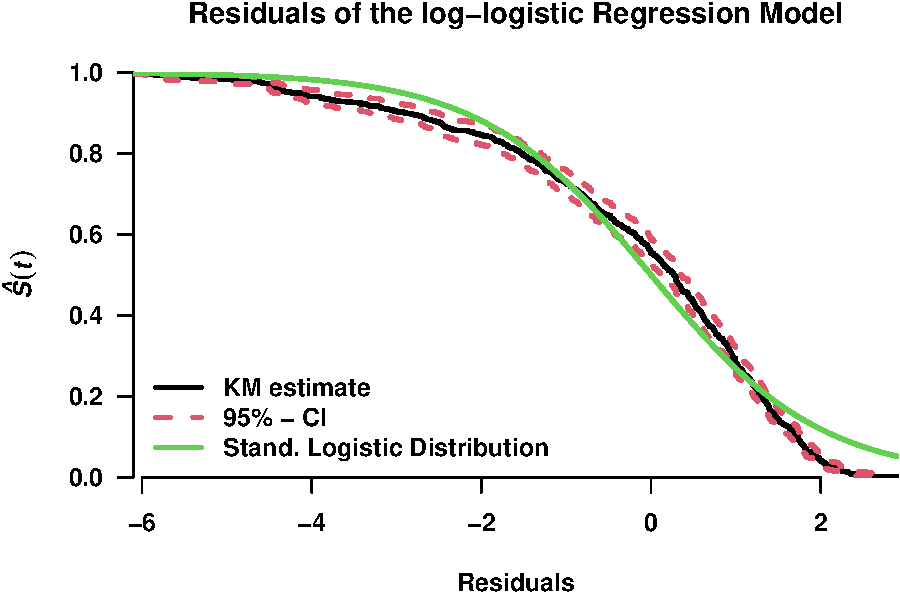
\includegraphics{practical_files/figure-latex/unnamed-chunk-13-1.pdf}

\begin{Shaded}
\begin{Highlighting}[]
\CommentTok{\# Weibull}
\FunctionTok{par}\NormalTok{(}\AttributeTok{font =} \DecValTok{2}\NormalTok{, }\AttributeTok{font.axis =} \DecValTok{2}\NormalTok{, }\AttributeTok{font.lab =} \DecValTok{2}\NormalTok{, }\AttributeTok{las =} \DecValTok{1}\NormalTok{, }\AttributeTok{mar =} \FunctionTok{c}\NormalTok{(}\DecValTok{5}\NormalTok{, }\DecValTok{5}\NormalTok{, }\DecValTok{4}\NormalTok{, }\DecValTok{2}\NormalTok{))}
\FunctionTok{plot}\NormalTok{(}\FunctionTok{survfit}\NormalTok{(}\FunctionTok{Surv}\NormalTok{(resids.weibull, std\_data}\SpecialCharTok{$}\NormalTok{cens) }\SpecialCharTok{\textasciitilde{}} \DecValTok{1}\NormalTok{), }\AttributeTok{col =} \FunctionTok{c}\NormalTok{(}\DecValTok{1}\NormalTok{,}\DecValTok{2}\NormalTok{,}\DecValTok{2}\NormalTok{), }\AttributeTok{xlab =} \StringTok{"Residuals"}\NormalTok{,}
     \AttributeTok{ylab =} \FunctionTok{expression}\NormalTok{(}\FunctionTok{bolditalic}\NormalTok{(}\FunctionTok{hat}\NormalTok{(S)(t))),}
     \AttributeTok{lty =} \DecValTok{1}\NormalTok{, }\AttributeTok{lwd =} \DecValTok{3}\NormalTok{, }\AttributeTok{yaxs =} \StringTok{"i"}\NormalTok{, }\AttributeTok{xaxs =} \StringTok{"i"}\NormalTok{, }\AttributeTok{bty =} \StringTok{"n"}\NormalTok{)}
\FunctionTok{title}\NormalTok{(}\StringTok{"Residuals of the Weibull Regression Model"}\NormalTok{)}
\NormalTok{survgumb }\OtherTok{\textless{}{-}} \ControlFlowTok{function}\NormalTok{(x) \{}
  \FunctionTok{return}\NormalTok{(}\FunctionTok{exp}\NormalTok{(}\SpecialCharTok{{-}}\FunctionTok{exp}\NormalTok{(x)))}
\NormalTok{\}}
\FunctionTok{curve}\NormalTok{(survgumb, }\AttributeTok{from =} \FunctionTok{min}\NormalTok{(resids.weibull), }\AttributeTok{to =} \FunctionTok{max}\NormalTok{(resids.weibull), }\AttributeTok{col =} \DecValTok{3}\NormalTok{, }\AttributeTok{lwd =} \DecValTok{3}\NormalTok{,}
      \AttributeTok{add =} \ConstantTok{TRUE}\NormalTok{)}
\FunctionTok{legend}\NormalTok{(}\StringTok{"bottomleft"}\NormalTok{, }\FunctionTok{c}\NormalTok{(}\StringTok{"KM estimate"}\NormalTok{, }\StringTok{"95\% {-} CI"}\NormalTok{, }\StringTok{"Stand. Gumbel Distribution"}\NormalTok{),}
       \AttributeTok{col =} \FunctionTok{c}\NormalTok{(}\DecValTok{1}\NormalTok{, }\DecValTok{2}\NormalTok{, }\DecValTok{3}\NormalTok{), }\AttributeTok{lty =} \FunctionTok{c}\NormalTok{(}\DecValTok{1}\NormalTok{, }\DecValTok{2}\NormalTok{, }\DecValTok{1}\NormalTok{), }\AttributeTok{lwd =} \DecValTok{3}\NormalTok{, }\AttributeTok{bty =} \StringTok{"n"}\NormalTok{)}
\end{Highlighting}
\end{Shaded}

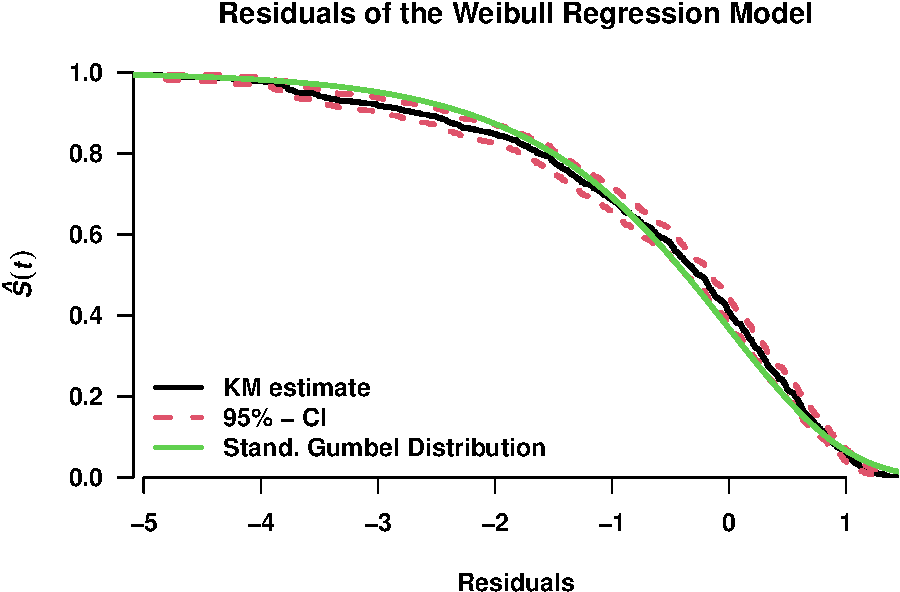
\includegraphics{practical_files/figure-latex/unnamed-chunk-13-2.pdf}

\begin{Shaded}
\begin{Highlighting}[]
\CommentTok{\# Log{-}normal}
\FunctionTok{par}\NormalTok{(}\AttributeTok{font =} \DecValTok{2}\NormalTok{, }\AttributeTok{font.axis =} \DecValTok{2}\NormalTok{, }\AttributeTok{font.lab =} \DecValTok{2}\NormalTok{, }\AttributeTok{las =} \DecValTok{1}\NormalTok{, }\AttributeTok{mar =} \FunctionTok{c}\NormalTok{(}\DecValTok{5}\NormalTok{, }\DecValTok{5}\NormalTok{, }\DecValTok{4}\NormalTok{, }\DecValTok{2}\NormalTok{))}
\FunctionTok{plot}\NormalTok{(}\FunctionTok{survfit}\NormalTok{(}\FunctionTok{Surv}\NormalTok{(resids.logno, std\_data}\SpecialCharTok{$}\NormalTok{cens) }\SpecialCharTok{\textasciitilde{}} \DecValTok{1}\NormalTok{), }\AttributeTok{col =} \FunctionTok{c}\NormalTok{(}\DecValTok{1}\NormalTok{,}\DecValTok{2}\NormalTok{,}\DecValTok{2}\NormalTok{), }\AttributeTok{xlab =} \StringTok{"Residuals"}\NormalTok{,}
     \AttributeTok{ylab =} \FunctionTok{expression}\NormalTok{(}\FunctionTok{bolditalic}\NormalTok{(}\FunctionTok{hat}\NormalTok{(S)(t))),}
     \AttributeTok{lty =} \DecValTok{1}\NormalTok{, }\AttributeTok{lwd =} \DecValTok{3}\NormalTok{, }\AttributeTok{yaxs =} \StringTok{"i"}\NormalTok{, }\AttributeTok{xaxs =} \StringTok{"i"}\NormalTok{, }\AttributeTok{bty =} \StringTok{"n"}\NormalTok{)}
\FunctionTok{title}\NormalTok{(}\StringTok{"Residuals of the Lognormal Regression Model"}\NormalTok{)}
\FunctionTok{curve}\NormalTok{(}\FunctionTok{pnorm}\NormalTok{(x, }\AttributeTok{lower.tail =}\NormalTok{ F), }\AttributeTok{from =} \FunctionTok{min}\NormalTok{(resids.logno), }\AttributeTok{to =} \FunctionTok{max}\NormalTok{(resids.logno), }\AttributeTok{col =} \DecValTok{3}\NormalTok{, }\AttributeTok{lwd =} \DecValTok{3}\NormalTok{,}
      \AttributeTok{add =} \ConstantTok{TRUE}\NormalTok{)}
\FunctionTok{legend}\NormalTok{(}\StringTok{"bottomleft"}\NormalTok{, }\FunctionTok{c}\NormalTok{(}\StringTok{"KM estimate"}\NormalTok{, }\StringTok{"95\% {-} CI"}\NormalTok{, }\StringTok{"Stand. Normal Distribution"}\NormalTok{),}
       \AttributeTok{col =} \FunctionTok{c}\NormalTok{(}\DecValTok{1}\NormalTok{, }\DecValTok{2}\NormalTok{, }\DecValTok{3}\NormalTok{), }\AttributeTok{lty =} \FunctionTok{c}\NormalTok{(}\DecValTok{1}\NormalTok{, }\DecValTok{2}\NormalTok{, }\DecValTok{1}\NormalTok{), }\AttributeTok{lwd =} \DecValTok{3}\NormalTok{, }\AttributeTok{bty =} \StringTok{"n"}\NormalTok{)}
\end{Highlighting}
\end{Shaded}

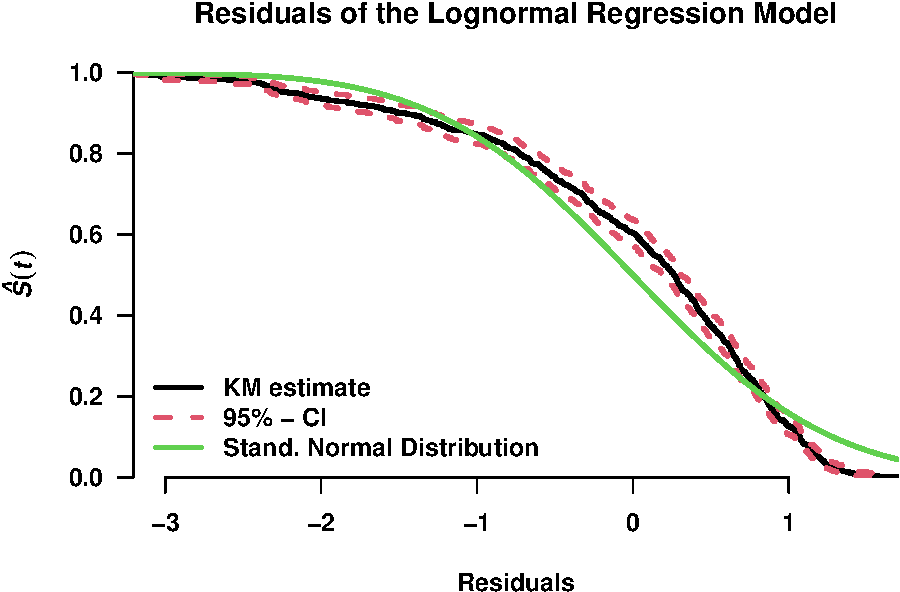
\includegraphics{practical_files/figure-latex/unnamed-chunk-13-3.pdf}

I would say that the Weibull looks the best based on the three residual plots that can be seen above. \textbf{But perhaps they should be tested in some other ways as well??}

Goodness of fit of the parametric models is done in lab6! These things can be used to choose which of the three distributions should be used!!

\begin{Shaded}
\begin{Highlighting}[]
\CommentTok{\# Does not really fit into the estimations from above! What have I done wrong?! I think I am misunderstanding something.}
\FunctionTok{cumhazPlot}\NormalTok{(std\_data}\SpecialCharTok{$}\NormalTok{TimeUntilReinf, std\_data}\SpecialCharTok{$}\NormalTok{cens,}\AttributeTok{col =} \DecValTok{4}\NormalTok{, }\AttributeTok{distr =} \FunctionTok{c}\NormalTok{(}\StringTok{"wei"}\NormalTok{, }\StringTok{"loglo"}\NormalTok{, }\StringTok{"lognormal"}\NormalTok{), }\AttributeTok{font.lab =} \DecValTok{4}\NormalTok{)}
\end{Highlighting}
\end{Shaded}

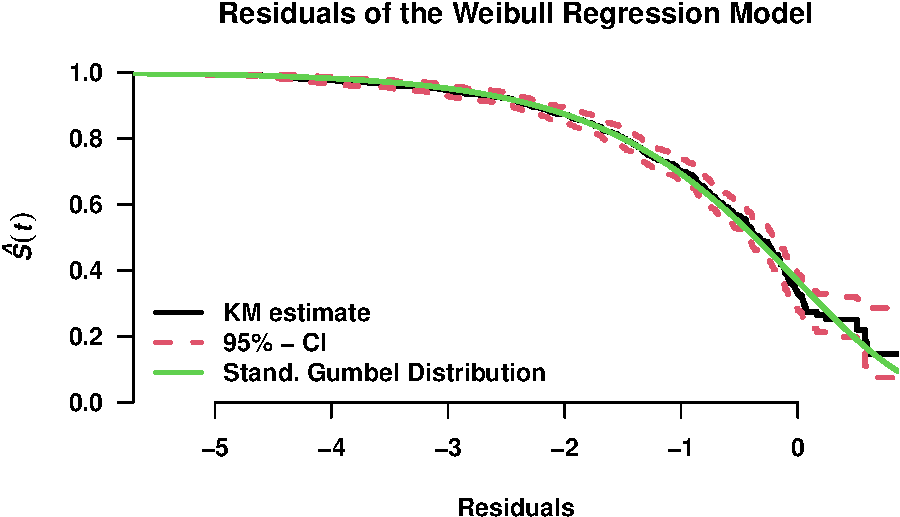
\includegraphics{practical_files/figure-latex/unnamed-chunk-14-1.pdf}

\begin{verbatim}
#> 
#> Parameter estimates
#> ===================
\end{verbatim}

\begin{verbatim}
#> $weibull
#>       shape       scale 
#>   0.8385125 340.1274020 
#> 
#> $loglogistic
#>      shape      scale 
#>   1.104856 198.683716 
#> 
#> $lognormal
#>  meanlog    sdlog 
#> 5.098800 1.637882
\end{verbatim}

Effect size measures:

\begin{itemize}
\tightlist
\item
  lognormal: acceleration factor.
\item
  weibull: HR.
\item
  log-logistic: OR.
\end{itemize}

\hypertarget{fit-of-a-semi-parametric-survival-model}{%
\section{Fit of a semi-parametric survival model}\label{fit-of-a-semi-parametric-survival-model}}

\hypertarget{conclusions}{%
\section{Conclusions}\label{conclusions}}

\end{document}
